\chapter{Results \& Discussion}\label{sec:ResultsAndDiscussion}

During the course of this project, an autonomous UGV for warehouse pick and place application was set up. Necessary mechanical modifications were done to the UGV platform in order to accommodate extra sensors and a robotic manipulator. Then, sensors and algorithms were configured to build a demonstration of how a warehouse application system could work with an autonomous UGV. Testing was then done separately on both the the autonomous navigation system and the pick and place system. Finally, the entire pipeline was tested, where autonomous navigation, machine vision and robot manipulation works together to achieve a warehouse automation task.

\section{Hardware}\label{R&D:Hardware}
As hardware aspects and some hardware design has been discussed in section \ref{sec:M:ConceptualDesign} \ref{sec:H:Hardware}, it is natural to include the result of the design process.

\subsection{Accessory Mounting Frame}\label{sec:R&D:H:AccessoryMountingFrame}
As mentioned in section \ref{sec:M:H:AccessoryMountingFrame}, an accessory mounting frame was made to accommodate auxiliary sensors and equipment. The frame is made out of $20X20[mm]$ aluminium strut profiles \cite{boshRexrothAluminium}, cut to length and put together according to the design in section \ref{sec:M:H:AccessoryMountingFrame}. \ref{sec:M:H:ANH:LidarAndCameraMount}, was fixed to the top of the accessory frame along with the OS1 LiDAR one camera. The complete physical UGV with the it's accessory frame including the LiDAR mount can be seen in figure \ref{fig:huskyComplete}.

\begin{figure}[ht]
  \centering
  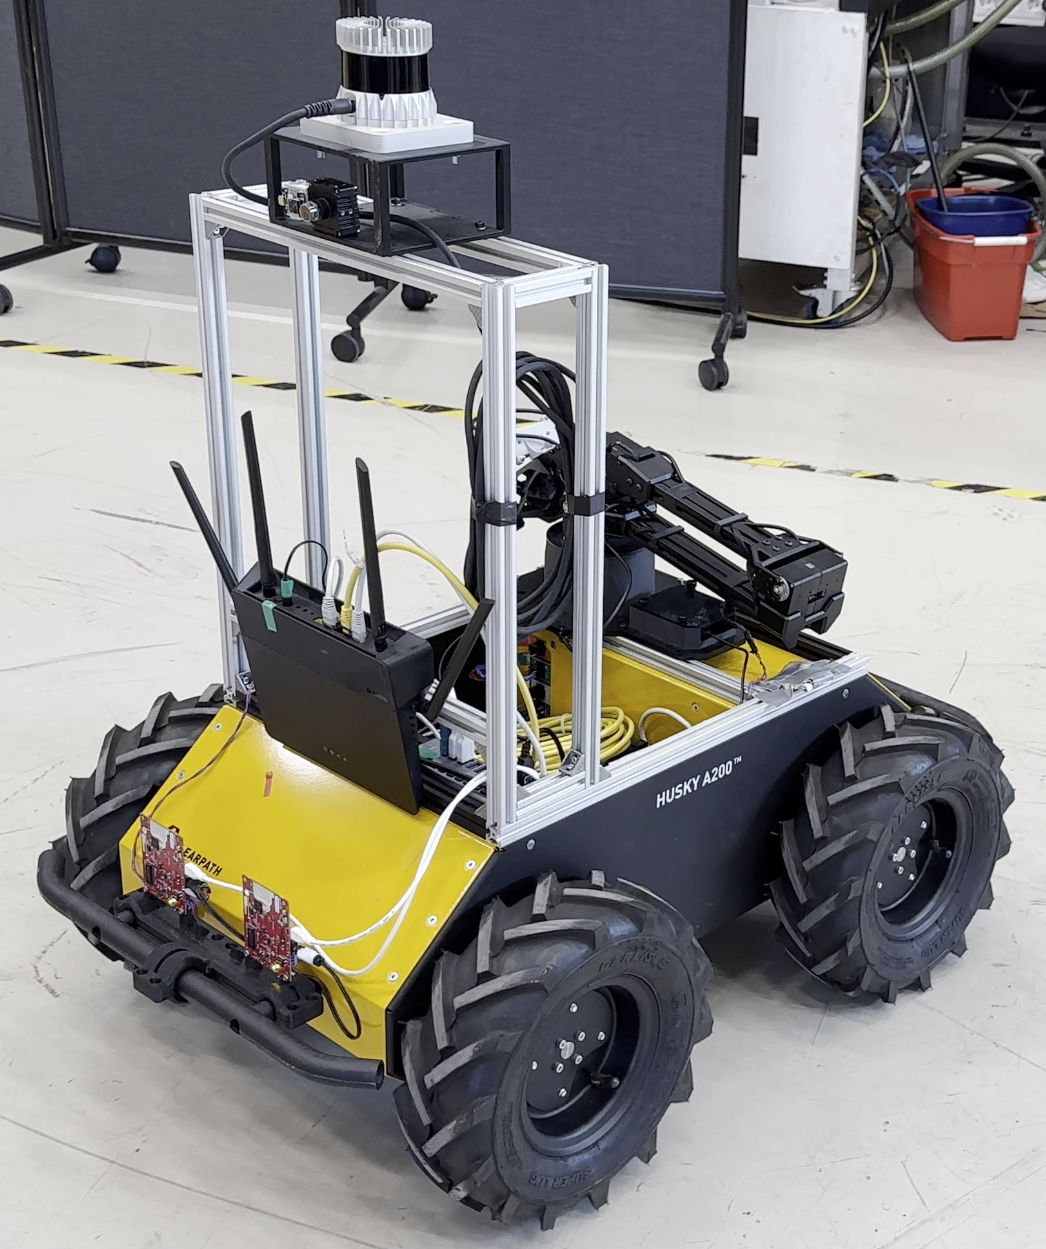
\includegraphics[width = 0.5\textwidth]{Figures/figHuskyComplete.png}
  \caption{Complete physical autonomous UGV configuration. The accessory mounting frame can be seen mounted on the Husky A200 UGV with the LiDAR mount including the OS1 LiDAR on top. Additionally, it can be seen that the VX300 manipulator is mounted in the rear right corner of the UGV.}
  \label{fig:huskyComplete}
\end{figure}

The accessory mounting frame has proven to be a practical and flexible solution that allows developers to mount various auxiliary equipment to the platform. 

\subsection{General Arrangement}\label{sec:R&D:GeneralArrangement}
Looking at figure \ref{fig:huskyComplete}, there is a radar mounting bracket with two Texas Instrument radars at the front of the Husky A200 UGV. This radar array is a part of another Master's Thesis by Didrik Robsrud running in parallel to this project. It is therefore not a part of the general arrangement drawing (figure \ref{fig:general_arrangement}) in section \ref{M:H:GeneralArrangement}. Apart from this radar array, the auxiliary components on the UGV is mounted in accordance to the general arrangement. All components are powered  through the Husky A200's power supply in accordance with the electrical interface drawing (figure \ref{fig:circuit_diagram}) in section \ref{M:H:ElectricalInterface}.

\subsection{Manipulator}\label{R&G:H:Manipulator}
The Interbotix VX300 manipulator, described in section \ref{sec:M:H:P&PH:Manipulator}, is mounted to the Husky A200 UGV in accordance with the description. An extra aluminium strut was added at the rear of the UGV to create extra mounting points for the manipulator. It can be seen how the manipulator is mounted on the husky in figure \ref{fig:huskyComplete}. 
This mounting position is practical in terms of packaging and keeping the manipulator within the confinements of the UGV while not in use. Nevertheless, the limited reach of the chosen manipulator resulted in a relatively small workspace outside the bounding box of the UGV. For example, the manipulator was unable to reach the ground, meaning that objects either has to be placed on an elevated surface, or the object has to be tall enough to be picked. This is unwanted as it places a higher demand on the accuracy of the autonomous navigation system. Additionally the limited reach of the manipulator results in less flexibility in therms of object placement at pick location.
Another consideration regarding the manipulator, is the absence of brakes of any kind in the manipulator's joints. This means that the servo motors constantly has to output a torque to hold a manipulator pose. One side effect of this is unnecessary power drainage, another is the fact that there are no safety mechanisms in place in case of power cut-off or sudden control system failure. In the case of a power cut-off or sudden control system failure, the manipulator could fall uncontrollably and possibly damage itself and/or its environment.

\subsection{Manipulator Mounted Camera}\label{R&D:H:ManipulatorMountedCamera}
As described in section \ref{sec:M:H:P&PH:ManipulatorMountedCamera}, a manipulator mounted camera has been set up. Section \ref{sec:M:H:P&PH:ManipulatorMountedCamera} also describes how this camera is mounted on the manipulator with a bracket designed for the task. The resulting configuration can be seen in figure \ref{fig:R&D:H:M:M:MMC:Vx300Complete}.

\begin{figure}[ht]
  \centering
  \begin{minipage}[b]{0.49\textwidth}
        \centering
        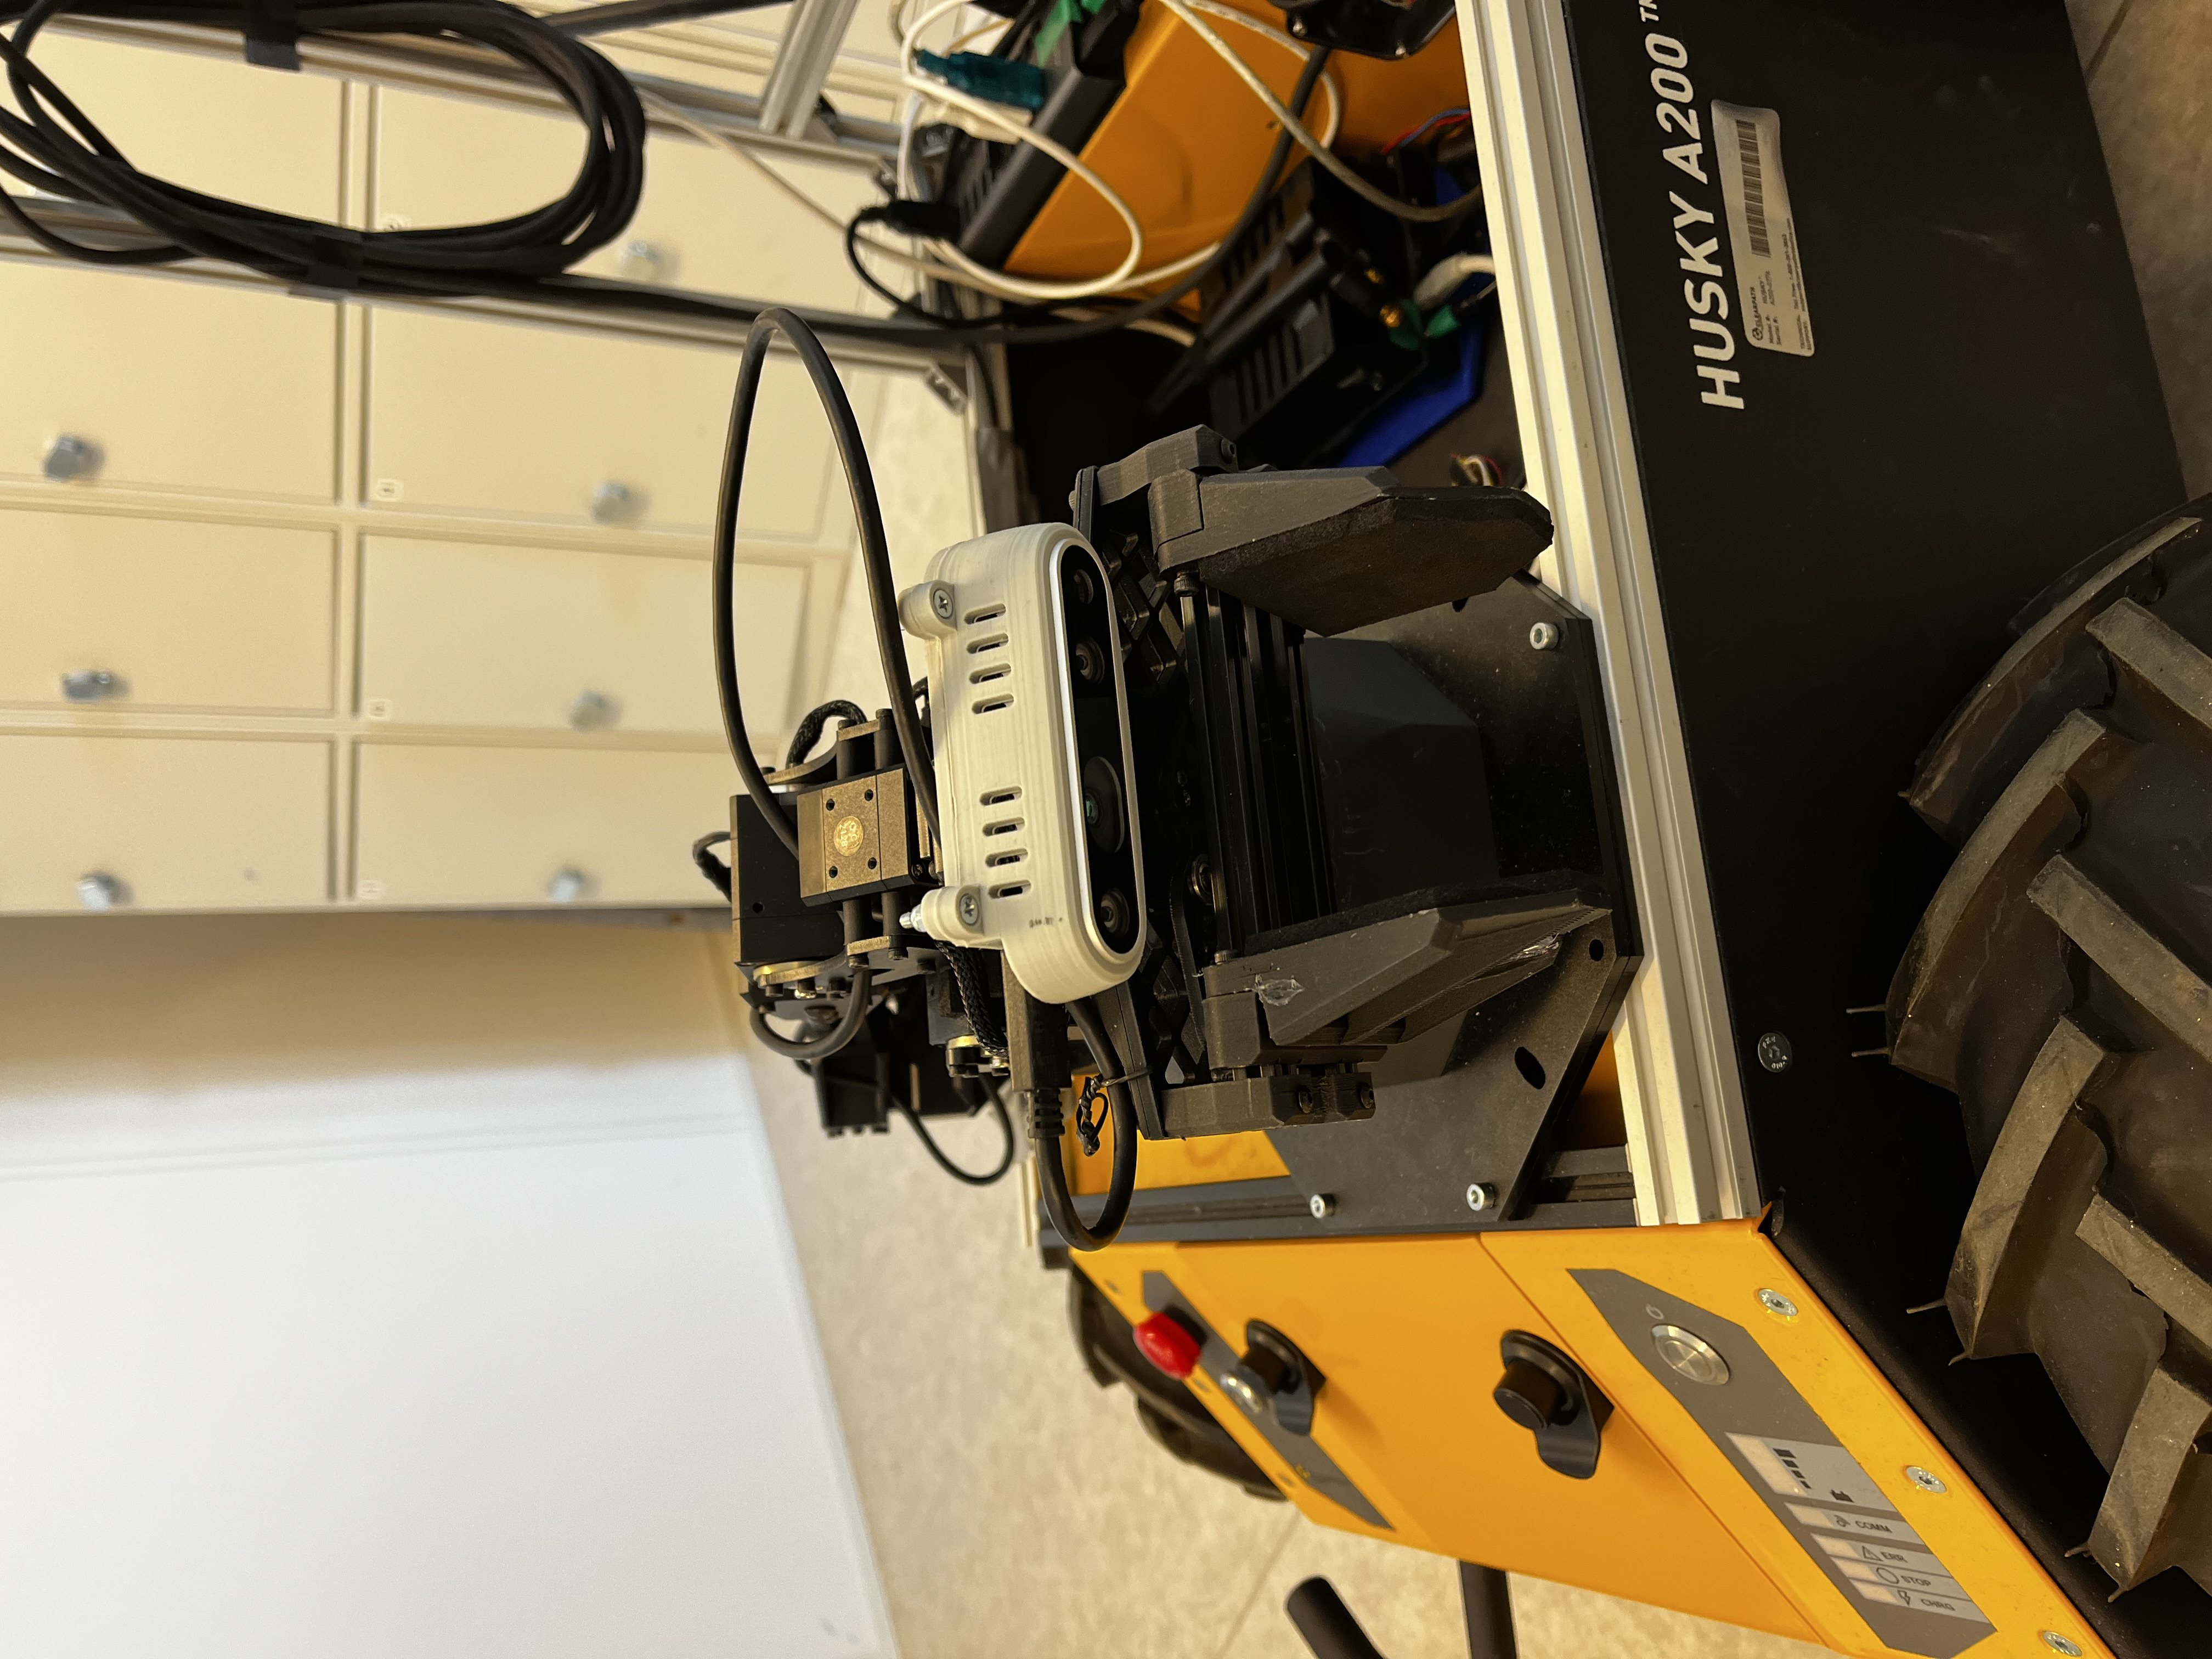
\includegraphics[angle=-90,width = 0.8\textwidth]{Figures/figVX300PhysComplete1.jpg}
  \end{minipage}
  \hfill
  \begin{minipage}[b]{0.49\textwidth}
    \centering
    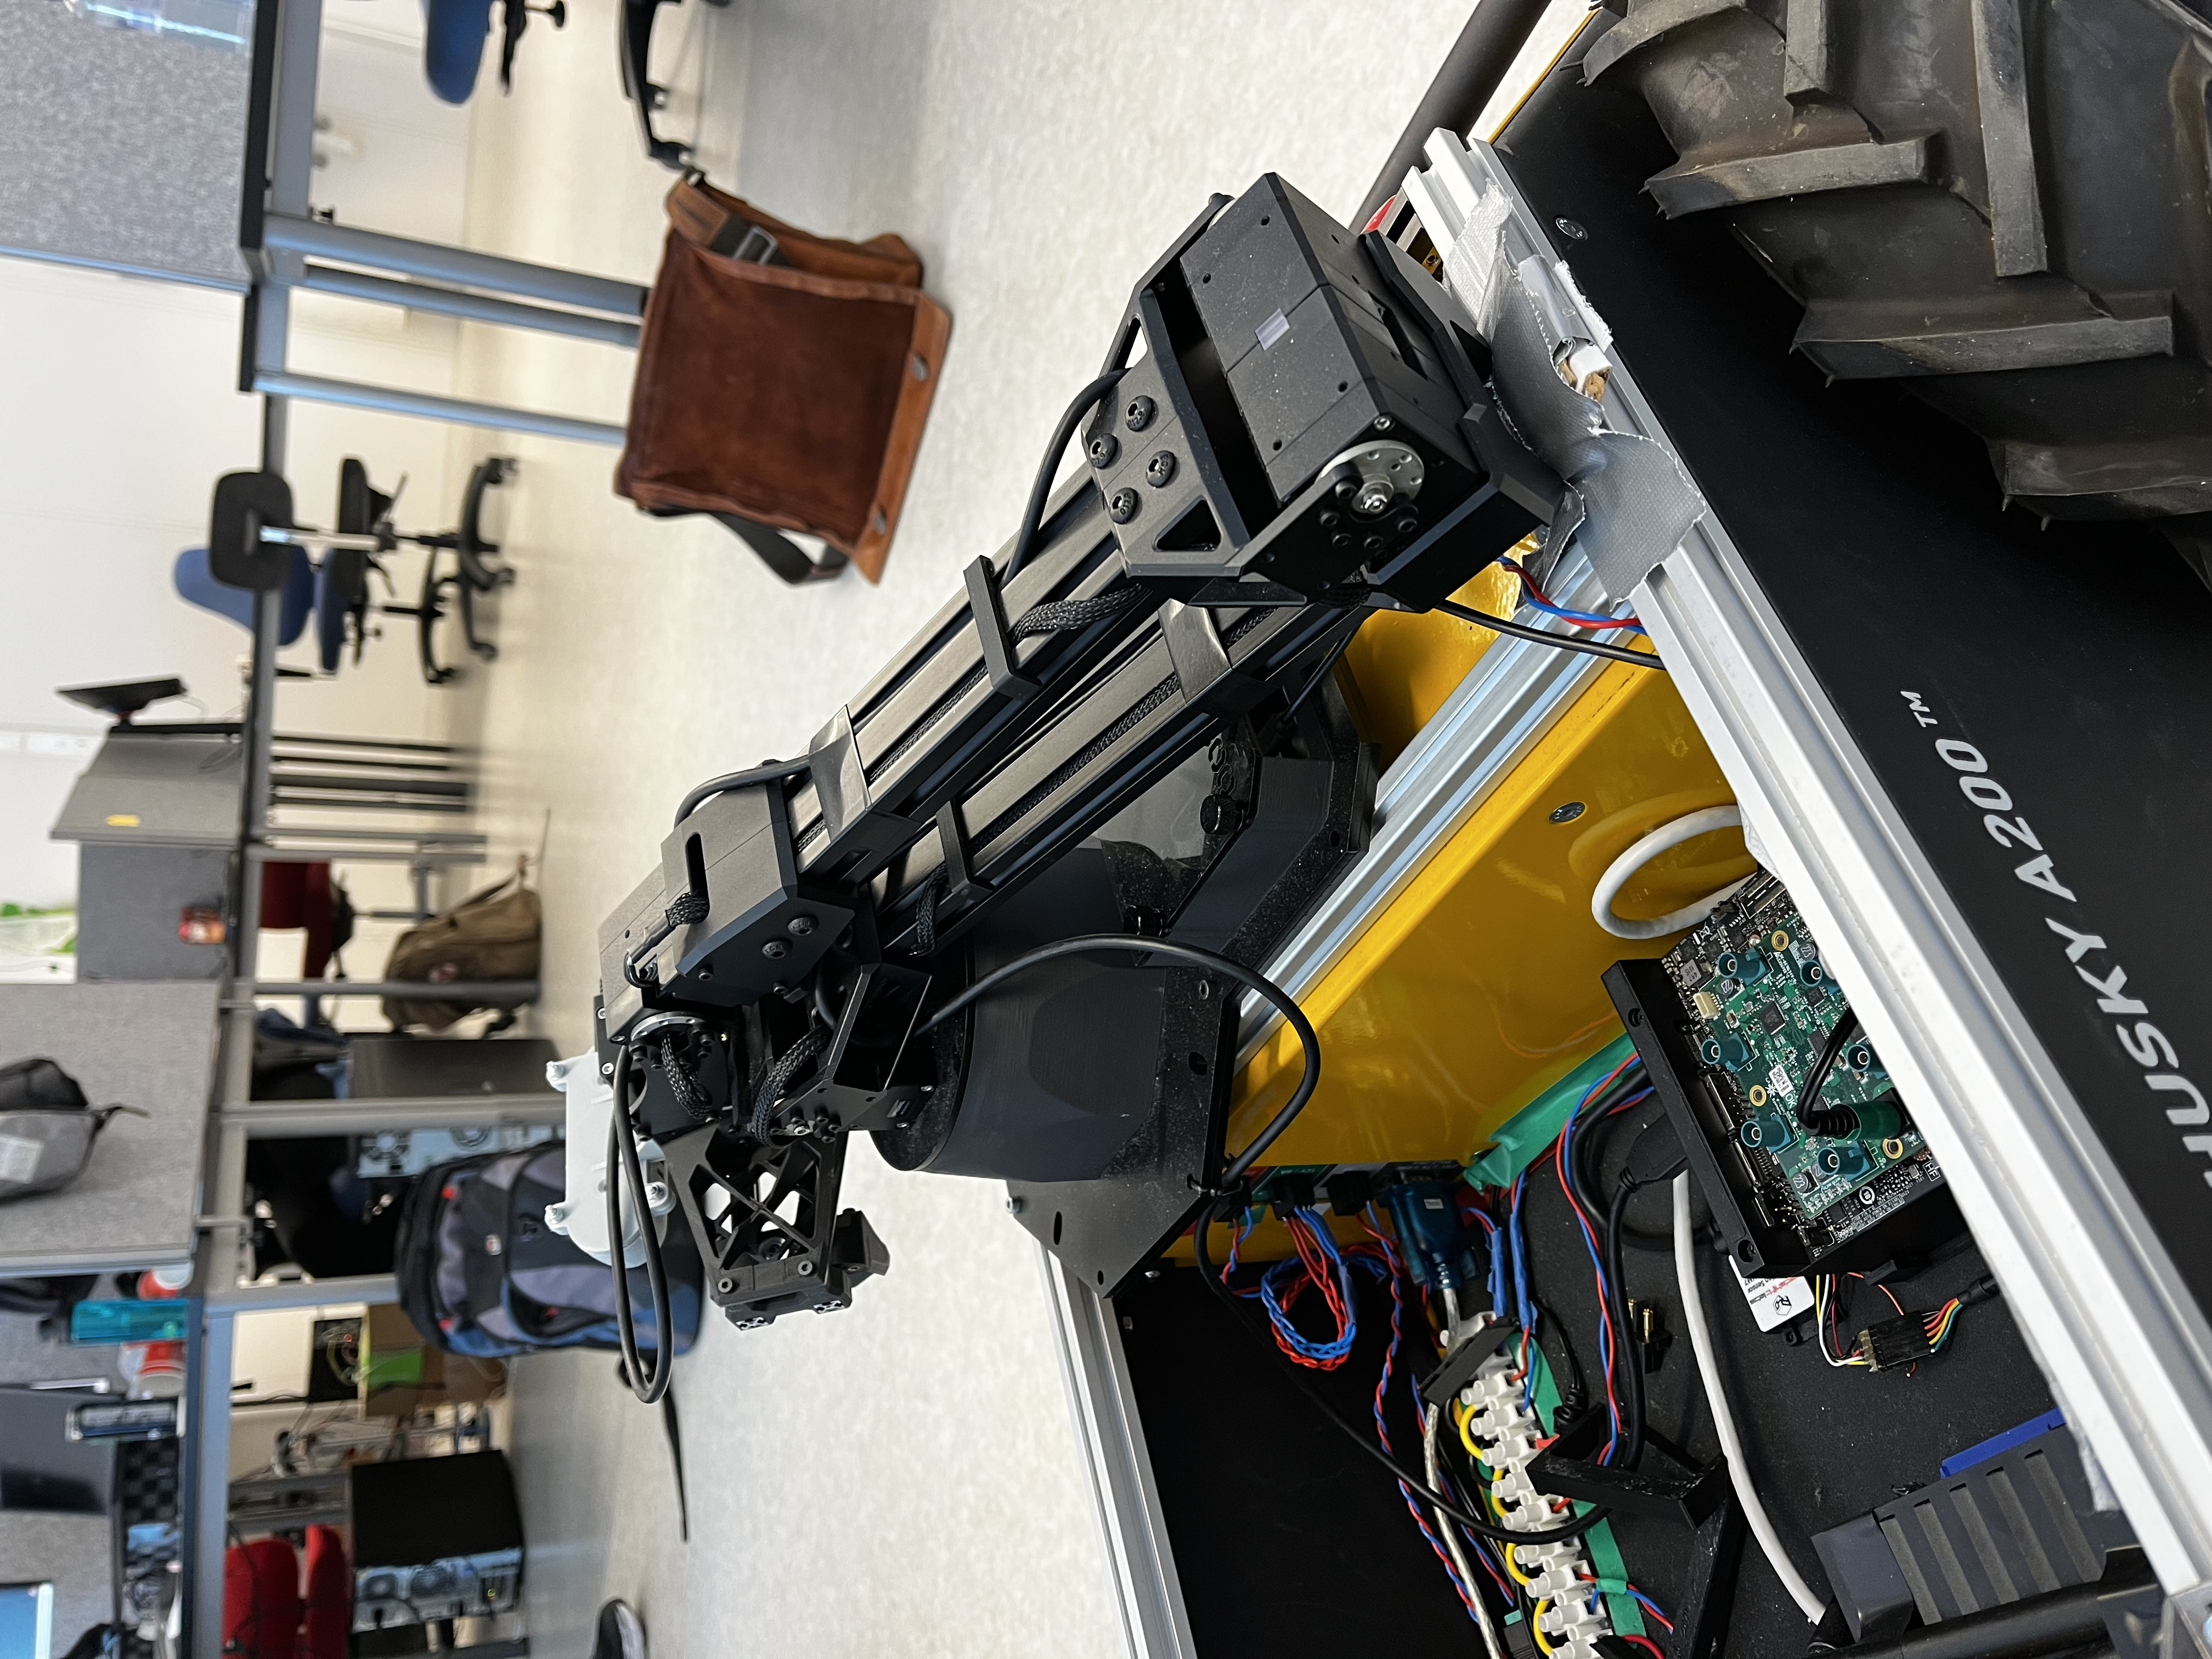
\includegraphics[angle=-90,width = 0.8\textwidth]{Figures/figVX300PhysComplete5.jpg}
  \end{minipage}
  \caption{Interbotix VX300 manipulator mounted on the Husky A200 UGV along with the manipulator mounted Realsense D435i camera. The Manipulator, although powered off in the image, receives it's power through the UGV's 12V power supply and controlled via an on-board Nvidia Jetson AGX Xavier Computer.}
  \label{fig:R&D:H:M:M:MMC:Vx300Complete}
\end{figure}

It is important that the pose of the camera is accurately defined and that the physical camera is fixed at the defined pose. The pose of the camera bracket is defined based on CAD measurements and can be assumed to be defined correctly. However, the pose of the camera relative to the bracket might not be accurately defined as this position was not thoroughly verified. The camera bracket seen in figure \ref{fig:R&D:H:M:M:MMC:Vx300Complete} proved to be successful at rigidly mounting the camera to the manipulator. However, inaccuracies in mounting pose relative to defined pose can not be ruled out due to possible slack in hole patterns at mounting flange.

\subsection{Digital Twin}
The complete configuration is set up with ROS2 so that a digital twin is possible to visualise in Rviz2. Compatibility with ROS2 allows for example visualisation of the robot on top of a 2D map while autonomously navigating through the environment. Figure \ref{fig:R&D:H:DigitalTwin:DigitalTwin} shows the digital twin visualised in Rviz2.

\begin{figure}[ht]
  \centering
  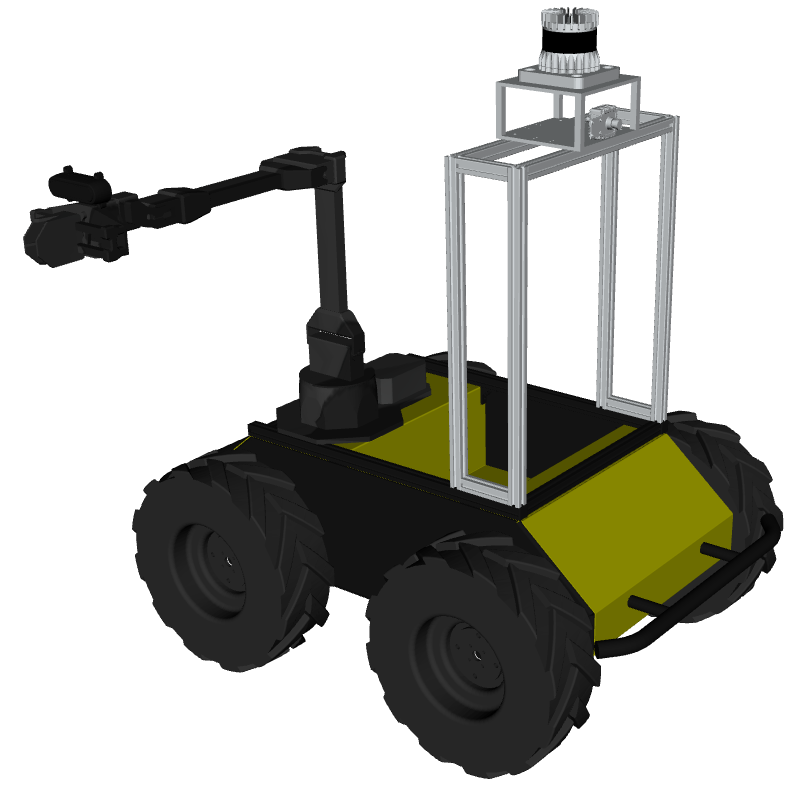
\includegraphics[width = 0.7\textwidth]{Figures/figDigitalTwin.png}
  \caption{Rviz2 visualisation of complete setup running in ROS2. This acts as a digital twin corresponding to the physical robot.}
  \label{fig:R&D:H:DigitalTwin:DigitalTwin}
\end{figure}

\section{Autonomous Navigation} \label{sec:R&D:AutonomousNavigaion}
The autonomous navigation is set up in ROS2 according to the descriptions in the method. In the context of this thesis, the UGV is a part of the autonomously navigating platform. Therefore the resulting configuration of the UGV will be described here. This section will present results regarding the autonomously navigating platform, starting with SLAM and then autonomous navigation results. All testing was preformed at UiA Campus Grimstad.

\section{Mobile Robot}\label{sec:R&D:Mobile Robot}
The Husky A200 UGV proved to be a practical mounting platform for developers to mount the equipment of their choice. However, there are some aspects of this UGV that should be discussed. The Husky A200 is a skidding robot (explained in section \ref{sec:T:AN:MRD:SkiddingRobots}), meaning that the robot will skid like a war-tank when turning. This is a major drawback when designing an autonomous robot since the skidding behaviour massively reduces the performance of the robot's odometry system. Sharp turns sometimes completely puts off the entire navigation system. 

% Efforts to reduce this issue has been made by using both the UM7 IMU and the LiDAR's built i IMU for dead reckoning and fusing this through an EKF. However, the UGV would still struggle, mainly when a goal position has been reached and the UGV would spin in place to correctly orient itself relative to the goal pose.

\section{Perception}
The Ouster OS1 LiDARs performance is affected by the high mounting location and it's relatively poor minimum range. The high mounting position creates a large blind-zone for low obstacles close to the robot. Ouster claims a vertical field of view of $45\deg$\textbf{SOURCE FOR THIS}, which at a sensor height of ...m above the ground means that 

The use of the ROS2 package \lstinline{pointcloud_to_laserscan}, described in section \ref{sec:M:AN:P:PointCloudToLaserScan} is considered a success as this resulted in a 2D mapping that took all relevant obstacles into account.

\subsection{Simultaneous Localisation and Mapping}\label{sec:R&D:AN:SLAM}
Testing of SLAM was done by running the complete UGV setup with SLAM and autonomous navigation. The SLAM algorithm would gen  map while travelling from the machine lab at campus to the elevators, this is a distance of about \textbf{DISTANCE}, and an area of about \textbf{AREA}. The resulting map can be seen in figure \ref{fig:R&D:AN:SLAM:figUiaMap}.

\begin{figure}[ht]
  \centering
  \includesvg[angle=90, width = 0.5\textwidth]{Figures/figUiaMap.svg}
  \caption{Map of Machine Lab and Corridor at UiA Campus Grimstad. The map has been generated through SLAM with an autonomous mobile robot.}
  \label{fig:R&D:AN:SLAM:figUiaMap}
\end{figure}

SLAM performance is considered to be acceptable, the resulting map, although not verified with a ground truth map, looks to be an accurate representation of the real world environments. 

\subsection{Navigation}\label{sec:R&D:AN:Navigation}
Navigation was tested by running the complete setup, together with SLAM, as mentioned in section \ref{sec:R&D:AN:SLAM}. As the map was generated on-the go, goal poses were manually updated by the operator as the map continued to be updated. Figure \ref{fig:R&D:H:SLAM:figNavUia} how the autonomous navigation is visualised on the operators computer using Rviz2.

\begin{figure}[ht]
  \centering
  \begin{minipage}[b]{0.49\textwidth}
        \centering
        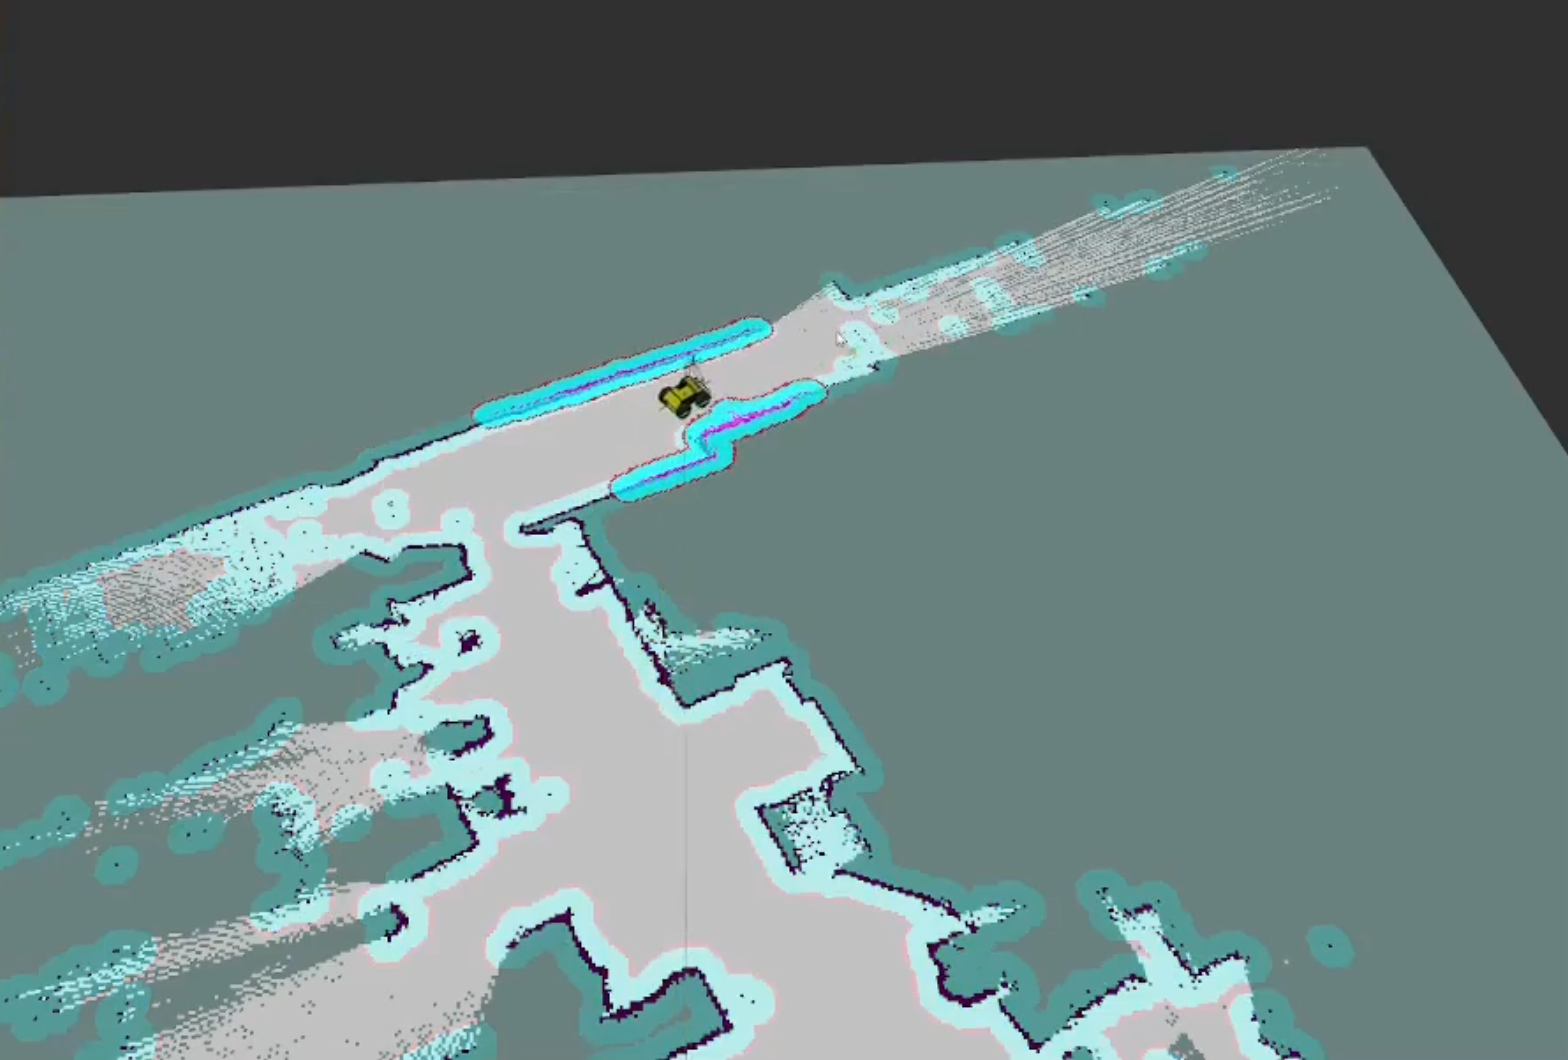
\includegraphics[width = 0.9\textwidth]{Figures/figNavUia2.png}
  \end{minipage}
  \hfill
  \begin{minipage}[b]{0.49\textwidth}
    \centering
    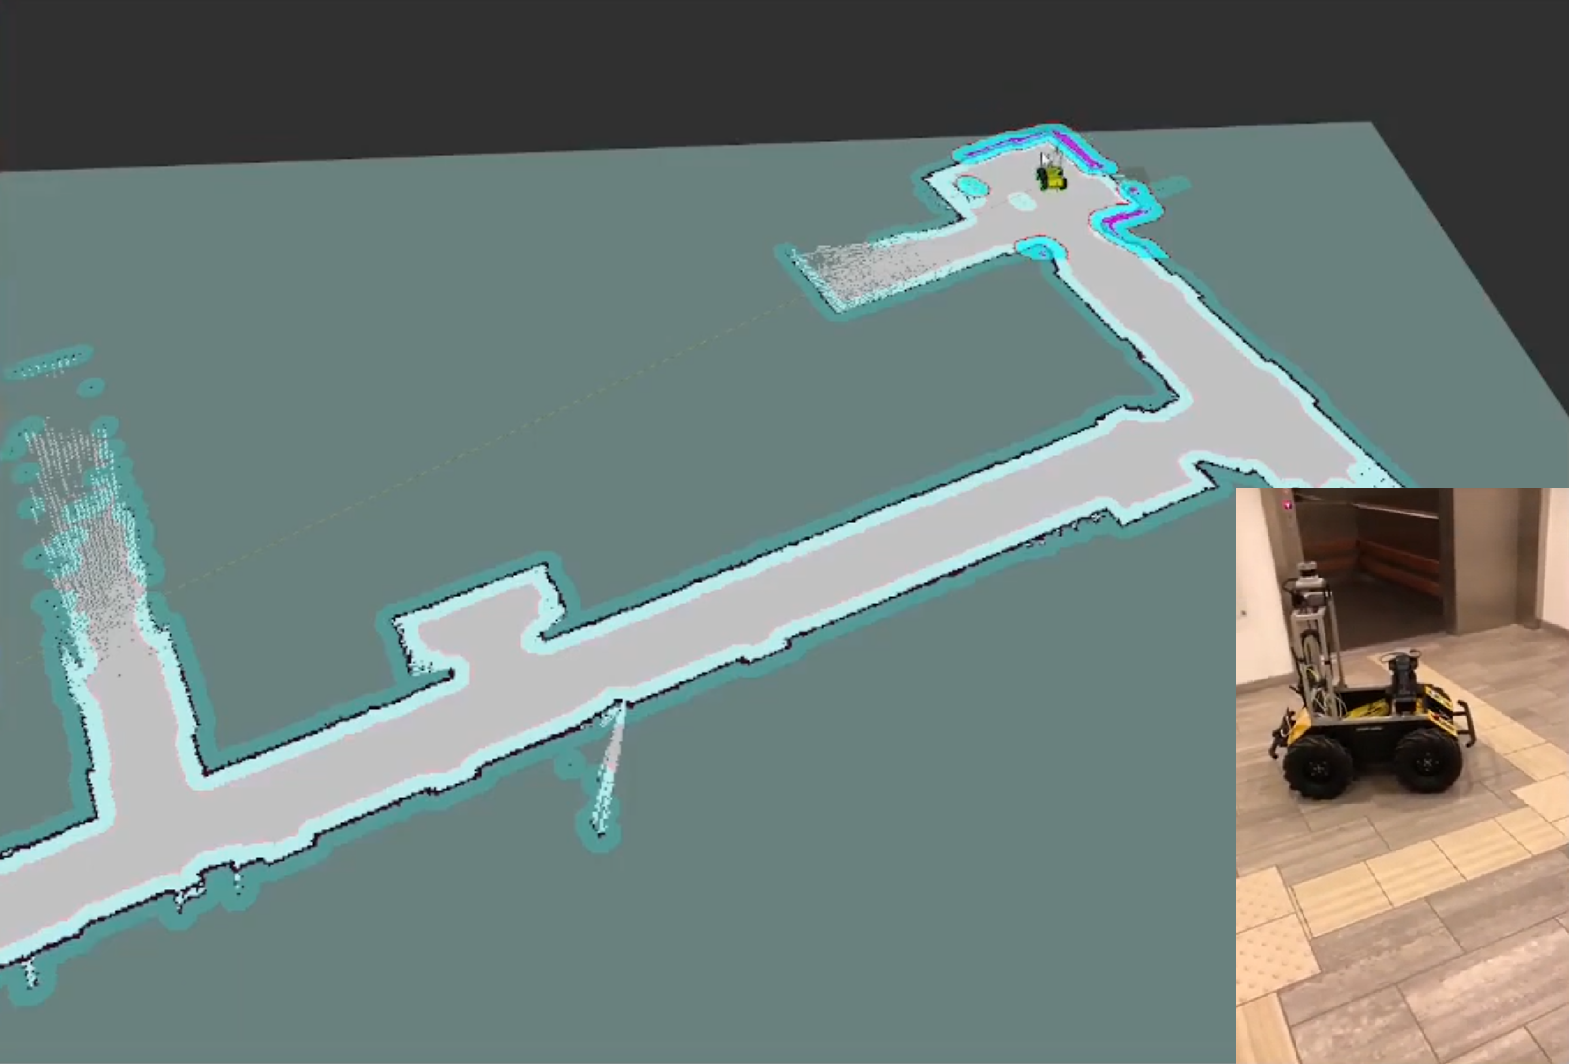
\includegraphics[width = 0.9\textwidth]{Figures/figNavUia4.png}
  \end{minipage}
  \caption{Mobile robot Running NAV2 along with SLAM on ROS2. This is a visualisation of Rviz2 where the mobile robot is illustrated as a 3D model on top of the generated map.}
  \label{fig:R&D:H:SLAM:figNavUia}
\end{figure}


\subsection{Collision Avoidance}
During navigation testing, collision avoidance was tested placing a person in front of the robot. Figure \ref{fig:R&D:H:CA:CollisionAvoidance1} and \ref{fig:R&D:H:CA:collisionAvoidance2} is taken from the Rviz2 visualisation of the navigation system, showing this test. In figure \ref{fig:R&D:H:CA:CollisionAvoidance1} the robot is moving without anything in it's way. A few moments later, a pedestrian has moved in front of the robot and the robot therefore has to plan around the pedestrian this can be seen in figure \ref{fig:R&D:H:CA:collisionAvoidance2}.

\begin{figure}[ht]
  \centering
  \begin{minipage}[b]{0.49\textwidth}
        \centering
        \includegraphics[width = 0.9\textwidth]{Figures/figuiaCollisionAvoid3.png}
        \caption{Robot navigating through a hallway. After this, a pedestrian will move in front of the robot and be detected by the local cost-map. Notice how the trajectory (green line) goes straight towards the goal.}
        \label{fig:R&D:H:CA:CollisionAvoidance1}
  \end{minipage}
  \hfill
  \begin{minipage}[b]{0.49\textwidth}
    \centering
    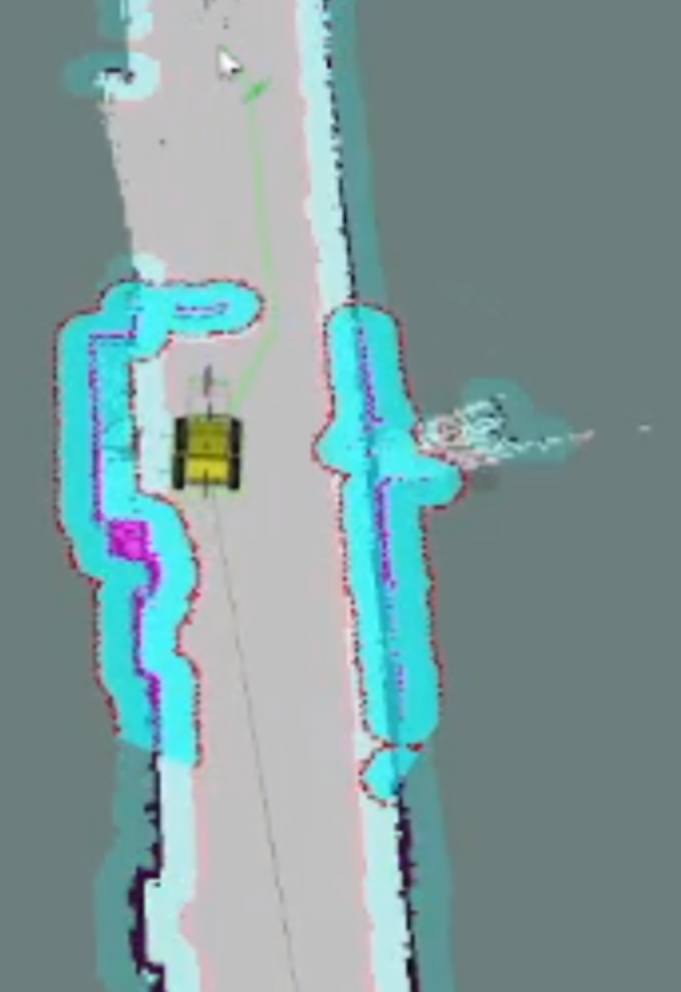
\includegraphics[width = 0.86\textwidth]{Figures/figUiaCollisionAvoid4.png}
    \caption{Robot navigating around obstacle. In this figure, a pedestrian is standing in the way of the robot, it therefore has to navigate around it. Notice how the trajectory (green line) goes around the object.}
    \label{fig:R&D:H:CA:collisionAvoidance2}
  \end{minipage}
\end{figure}


\section{Pick and Place} \label{R&D:PickAndPlace}
Pick and place operations is achieved through a combination of three systems. The first system is the VX300 manipulator itself and it's ROS2 Moveit2 packages described in section \ref{sec:M:MRC:Manipulator}. The second system is the machine vision system described in section \ref{sec:M:MRC:MachineVision}. This includes the vision camera, its drivers and the AprilTag based object detection system. The last system needed is the custom pick and place ROS2 package described in section \ref{sec:M:A:HuskyPickAndPlace}. The performance of the manipulator will not be discussed, as it can be assumed that the manipulator preforms as intended using the ROS2 packages provided by the manufacturer. Therefore, only results regarding object detection and the custom pick and place ROS2 package will be presented.


\subsection{Object Detection \& Pick and Place}
The tag based machine vision system was set up according to section \ref{sec:M:MRC:MachineVision}. The performance of the vision system is verified by testing the combined pick and place performance of the manipulator. Interbotix states a repeatability of 1[mm] for the manipulator\cite{interbotix_vx300}. This tells that variations in pick and place performance outside this measure could be attributed to the vision system.

\subsection{Custom Scene Publisher Package}
As mentioned in section \ref{sec:M:A:SceneGeometryPublisher}, a custom ROS2 package was made to publish collision boxes to the planning scene. The package is made to be able to read a ".scene" file generated from Rviz2 and then publish the information from this file to the planning scene. The package is run automatically when launching the manipulator using the custom launch file \lstinline{xavier2_launch.py} from the git repository made for this projects manipulator\cite{husky_vx300_repo}. An example of this is given in figure \ref{fig:R&D:P&P:CSP:scenePublisher1} and  \ref{fig:R&D:P&P:CSP:scenePublisher2} where the manipulator has first been initiated in an empty space in figure \ref{fig:R&D:P&P:CSP:scenePublisher1}, then the package has been launched and the collision boxes that encapsulate the robot has been published in figure \ref{fig:R&D:P&P:CSP:scenePublisher2}. These collision boxes are usually hidden in Rviz2 in favour of nicer visuals shown in section \ref{fig:R&D:H:DigitalTwin:DigitalTwin}.

\begin{figure}[ht]
  \centering
  \begin{minipage}[b]{0.49\textwidth}
        \centering
        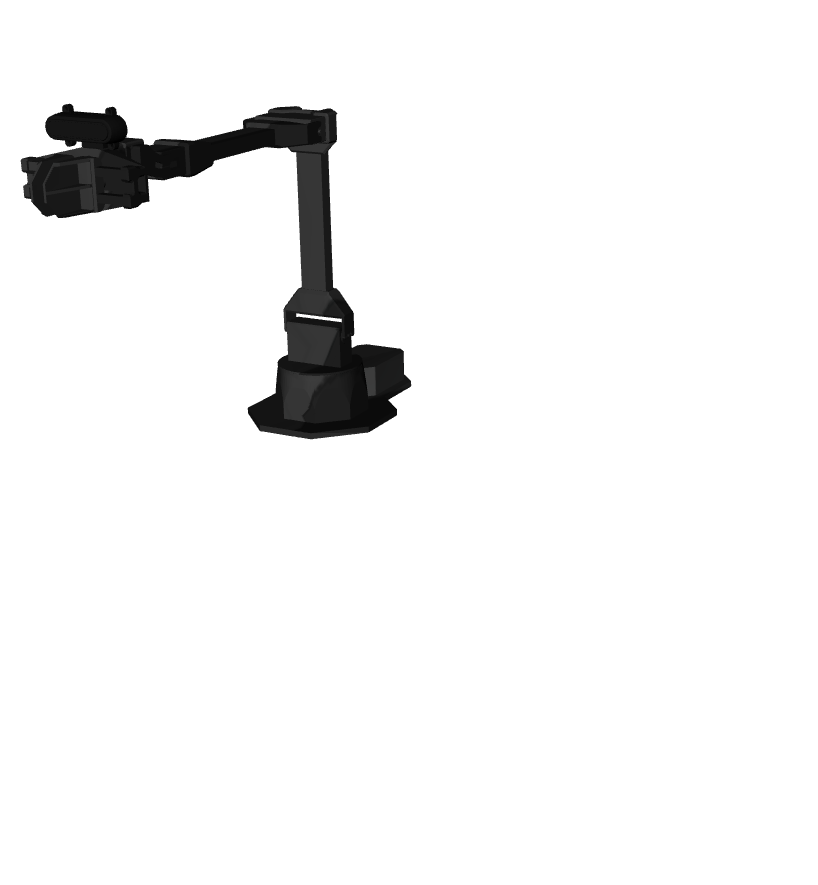
\includegraphics[width = 0.9\textwidth]{Figures/figScenePublisher1.png}
        \caption{Manipulator initiated with Moveit2 and visualised in Rviz2. In this configuration, the Manipulator would not know about the UGV and collisions could occur.}
        \label{fig:R&D:P&P:CSP:scenePublisher1}
  \end{minipage}
  \hfill
  \begin{minipage}[b]{0.49\textwidth}
    \centering
    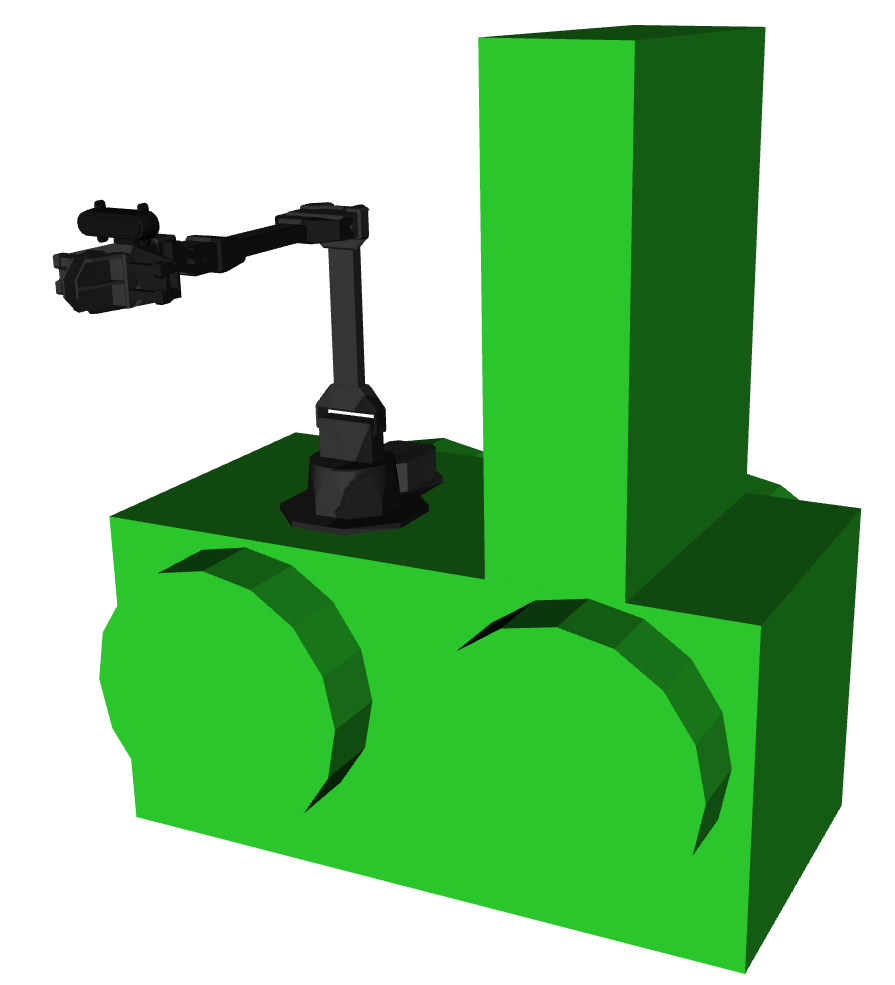
\includegraphics[width = 0.86\textwidth]{Figures/figScenePublisher2.png}
    \caption{Manipulator initiated with Moveit2 and visualised in Rviz2. Collision boxes are published to the planning scene using the custom Scene Publisher ROS2 package. The manipulator will not collide with the UGV in this configuration.}
    \label{fig:R&D:P&P:CSP:scenePublisher2}
  \end{minipage}
\end{figure}


\subsection{Custom Pick and Place Package}
A custom ROS2 package has been made to enable control of the manipulator and get feedback about current operation through the ROS2 network's topic system. The design of this package is described in section \ref{sec:M:A:HuskyPickAndPlace}. Testing has been done to tune the robot's move sequences and to verify the robustness of the ROS2 topic based command and feedback system. 

\textbf{Do some testing and write a bit about it here}



\section{Warehouse Automation}
The full warehouse automation pipeline is set up using the custom ROS2 package described in section \ref{sec:M:A:HuskyMasterNode}. Running this package results in the UGV autonomously navigating to a predefined pick location before running the pick operation. The pick operation includes using machine vision to detect and estimate the pose of the object before picking. After picking, the UGV moves to the place location and the place operation is preformed. Finally, the UGV will return to it's starting position.




%aj \section{experiment}
% write about different environment where experiment is done

% \subsection{indoor environment}

% \subsection{ware house environment}

% \section{Results}
% write that algorithms in ch 3.. was implemented to get the results with accuracy and precision, error ...

% KPI for each of functionality - show that it could navigate without collision, localize and estimate the pose of object with error xxx, pick it and place it at predefined location with error xxx

% \section{Pick and Place}



% \section{Autonomous Navigation}
% Bad kinematic design on Husky

% \section{Tag Detection}
% Worked like a charm

% \section{Pick and Place}
% Small and weak manipulator

% \section{Husky Master}
%  Unpolished Algorithm

%  \section{Husky Pick and Place}
%  Unpolished algorithm
%  Not general
%  not ideal launch file
 
%  Two methods for picking were discussed. Both of these places restrictions on the pose/shape of the objects t be picked. One method of picking bases itself on picking the objects from the side. That is, the manipulator moves in from the side of the object when gripping it. This 

%  \section{Scene Geometry Publisher}
%  Not ideal launch file
%  General design, but not general launch

 %Conclusion and Discussion